\documentclass[review]{elsarticle}
\usepackage{comment}
\usepackage{url}
%
\usepackage[breaklinks]{hyperref}
\usepackage{breakurl}


\usepackage[ruled]{algorithm2e}

%\usepackage{lineno}
%\modulolinenumbers[5]

\journal{Optics Communications}

%%%%%%%%%%%%%%%%%%%%%%%
%% Elsevier bibliography styles
%%%%%%%%%%%%%%%%%%%%%%%
%% To change the style, put a % in front of the second line of the current style and
%% remove the % from the second line of the style you would like to use.
%%%%%%%%%%%%%%%%%%%%%%%

%% Numbered
%\bibliographystyle{model1-num-names}

%% Numbered without titles
%\bibliographystyle{model1a-num-names}

%% Harvard
%\bibliographystyle{model2-names.bst}\biboptions{authoryear}

%% Vancouver numbered
%\usepackage{numcompress}\bibliographystyle{model3-num-names}

%% Vancouver name/year
%\usepackage{numcompress}\bibliographystyle{model4-names}\biboptions{authoryear}

%% APA style
%\bibliographystyle{model5-names}\biboptions{authoryear}

%% AMA style
%\usepackage{numcompress}\bibliographystyle{model6-num-names}

%% `Elsevier LaTeX' style
\bibliographystyle{elsarticle-num}
%%%%%%%%%%%%%%%%%%%%%%%
\usepackage{graphicx}
\usepackage{subcaption}
%%%%%%%%%%%%%%%%%%%%%%%%%%%%%%%%%%%%%%%%%%%%%%%%%%%%%%%%%%%%%%%%%%%%%%%%%%%%%%%%%%

\usepackage[svgnames]{xcolor} % Enabling colors by their 'svgnames'

\usepackage{amsmath}
\usepackage{amsfonts}
\usepackage{amssymb}
%%%%%%%%%%%%%%%%%%%%%%%%%%%%%%%%%%%%%%%%%%%%%%%%%%%%%%%%%%%%%%%%%%%%%%%%%%%%%%%%%%

 
\begin{document} 

\begin{frontmatter}

\title{Illumination Level Independence in the Dynamic Laser Speckle Analysis}
%\tnotetext[mytitlenote]{Fully documented templates are available in the 
%elsarticle package on \href{http://www.ctan.org/tex-archive/macros/latex/contrib/elsarticle}{CTAN}.}



% Group authors per affiliation:
\author{-------- ------- ------}
\author{-------- ------- ------}



% \author{Fernando Pujaico Rivera\fnref{myfootnote2}}
% \author{Roberto Alves Braga Jr.\fnref{myfootnote1}}
% \address{University Federal of Lavras, Lavras, Brazil}
% \fntext[myfootnote2]{201518201@posgrad.ufla.br}
% \fntext[myfootnote1]{robertobraga@deg.ufla.br }


\begin{abstract}
In this article we show an analysis of how the frequency band,
of the speckle signal, influence in the
light independence of the speckle index value in a dynamic laser speckle analysis. 
Specifically, 
will be studied as It is influenced the temporal speckle deviation 
index by the use of 3 different frequency bands of the speckle signal.
Finally, It is shown as signals with high frequency values
return values with more illumination level independence.
\end{abstract}

\begin{keyword}
Biospeckle laser \sep 
Biospeckle index \sep 
Biospeckle signal\sep 
Biological activity \sep
Dynamic speckle \sep  
Backscattering.
\end{keyword}

\end{frontmatter}

\linenumbers

%%%%%%%%%%%%%%%%%%%%%%%%%%%%%%%%%%%%%%%%%%%%%%%%%%%%%%%%%%%%%%%%%%%%%%%%%%%%%%%%%%%%%%%%%
%%%%%%%%%%%%%%%%%%%%%%%%%%%%%%%%%%%%%%%%%%%%%%%%%%%%%%%%%%%%%%%%%%%%%%%%%%%%%%%%%%%%%%%%%
\section{Introduction}
In the literature we can found a work \cite{RIVERA2017144} that show as some speckle indexes
have a frequency filter behavior; by example, we have the $AVD$ \cite{avd} and 
$IM$ \cite{ARIZAGA1999163} index, that they filter
the information like a first order high pass filter with cut-off in the middle
of normalized frequency band. For this reason, It is important analyze how,
the chosen frequency band, alter the result of selected index.
By other side others works 
\textcolor{red}{[cita] (acho tinha um artigo de kefir que tinha problemas de iluminacao)} 
show the problem of
made a speckle analysis with the presence of variation of illumination, because
the most of biospeckle indexes in the literature are influenced in your values
by the use of a determinate illumination level.
Thus, the present work searches establish a relation between the frequency band used
and the speckle index; specifically here will be studied the dependence of
the temporal speckle deviation matrix \cite{Nothdurft:05} with the illumination level.


%%%%%%%%%%%%%%%%%%%%%%%%%%%%%%%%%%%%%%%%%%%%%%%%%%%%%%%%%%%%%%%%%%%%%%%%%%%%%%%%%%%%%%%%%
%%%%%%%%%%%%%%%%%%%%%%%%%%%%%%%%%%%%%%%%%%%%%%%%%%%%%%%%%%%%%%%%%%%%%%%%%%%%%%%%%%%%%%%%%
\section{System description}
\label{sec:description}

\subsection{Obtaining data packages in the test over an ink sample}
\label{sec:descriptionink}
The Fig. \ref{fig:system} shows the system diagram of the ink sample test; in It, we can see as
a red laser was pointed to an ink sample, the drying process is monitored by a digital camera;
the images are collected receiving two different illumination levels, because these 
are obtained using a neutral 
density lens between the ink sample and the laser, covering partially the view angle of the laser.
The images in each data package
are sampled with a frequency of $F_s=$\textcolor{red}{[[[12.5]]]} hertz, being 
collected $N=400$ images by package. In total were collected $11$ packages 
(with two different illumination levels each one) at the minutes 
$0$, $10$, $20$, $30$, $40$, $50$, $60$, $75$,$105$,$120$ and $150$ of drying process. 
\begin{figure}[ht!]
\centering
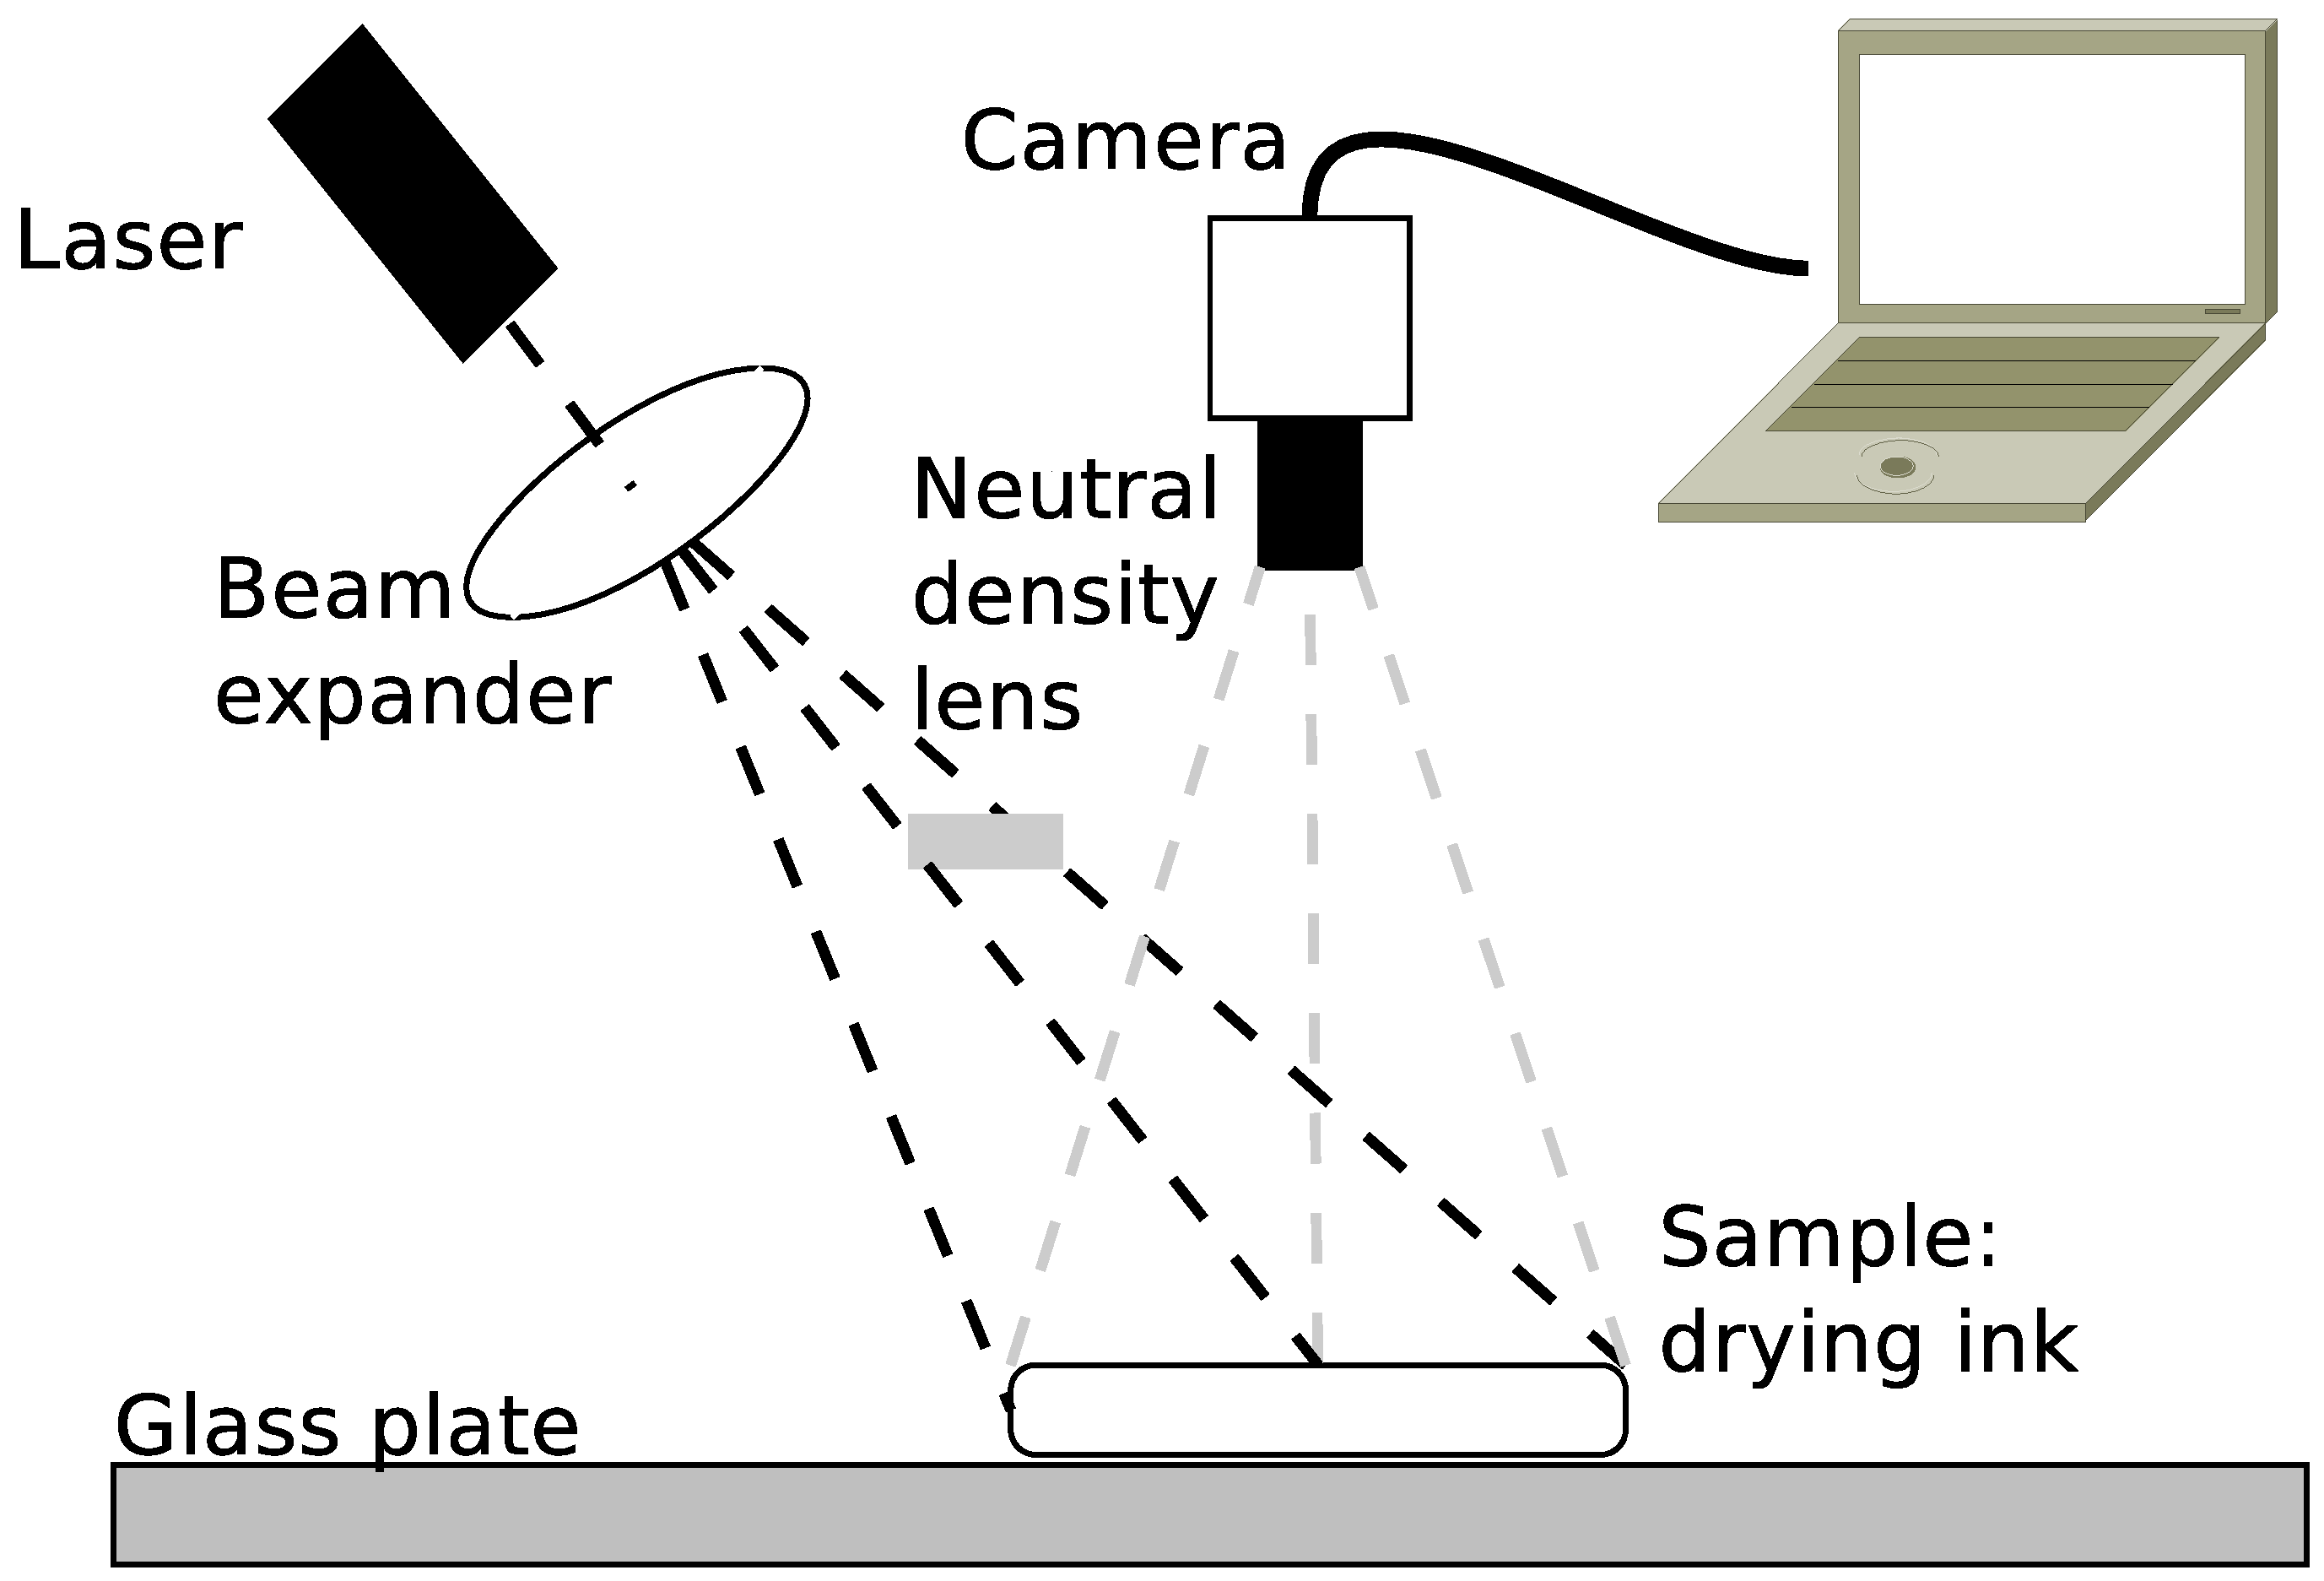
\includegraphics[width=0.65\columnwidth]{system.eps}
\caption{System description.}
\label{fig:system}
\end{figure}
In each one of the $11$ packages were selected two regions, of $250\times200$ pixels, 
corresponding to the regions with two different illumination levels, 
as shown with black lines in the Fig. \ref{fig:regions}. In the right side of the figure  we have the
portion of image that was altered by the neutral density lens. The figure represents
with a color bar the result of  calculus the temporal speckle mean matrix ($\mu$) according the Eq. (\ref{eq:cont1})
showed in the Sec. \ref{subsec:deviation}. Being this value associated in the literature with
the illumination quantity in the surface of sample \cite{Nothdurft:05}; corresponding thus high values of $\mu$
to places with more illumination. 
\begin{figure}[h!]
\centering
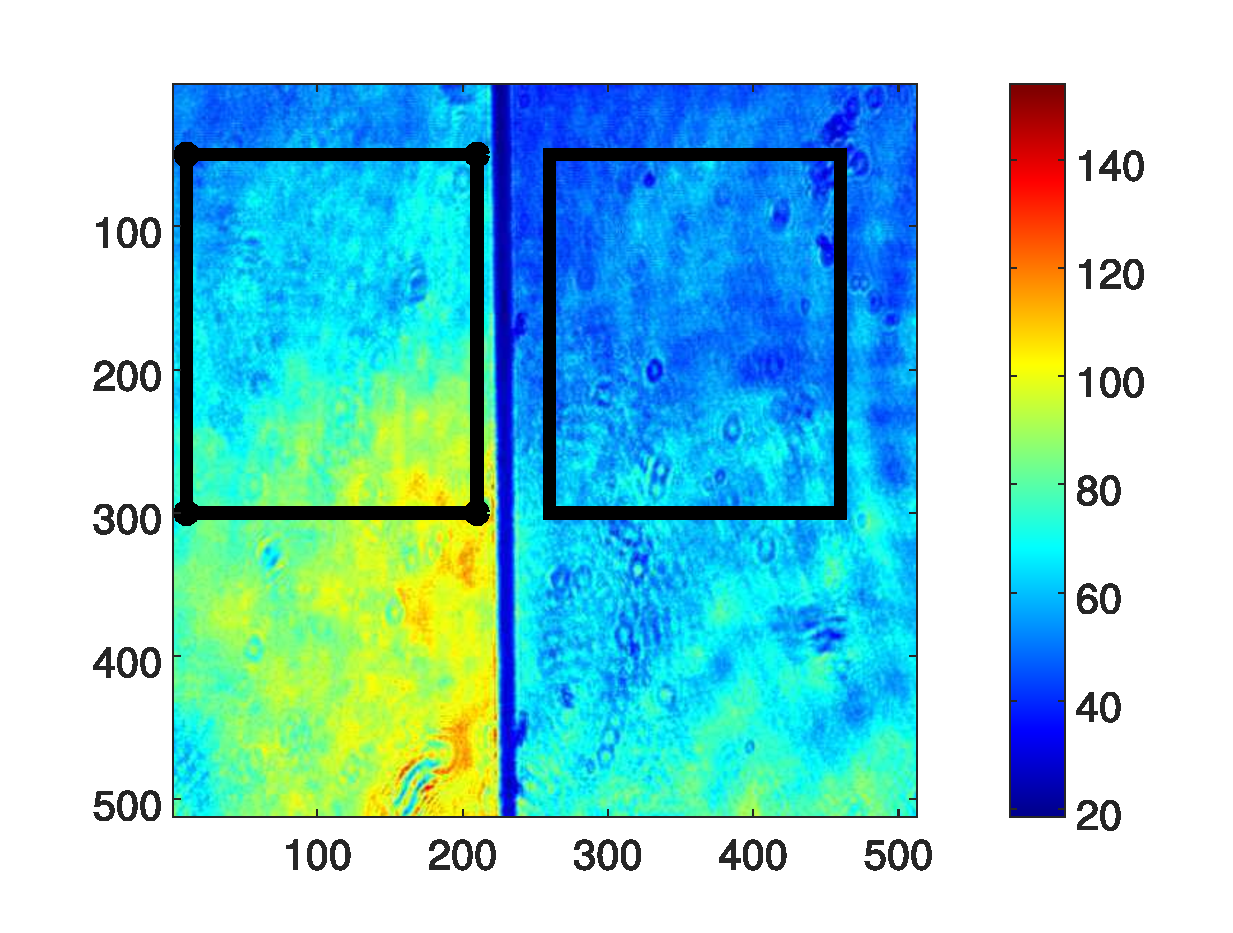
\includegraphics[width=0.85\columnwidth]{meanall_points_all.eps}
\caption{Selected regions and light intensity distribution in the ink drying test.}
\label{fig:regions}
\end{figure}

\subsection{Obtaining data packages in the test over a paper piece}
\label{sec:descriptionpaper}
The test over a paper piece has a similar configuration that seen in
the Fig. \ref{fig:system} with the difference that in the paper piece test is not used
the neutral density lens; thus It is collected one data package
sampled with a frequency of $F_s=$\textcolor{red}{[[[12.5]]]} hertz, being 
collected in total $N=129$ images of 640$\times$480 pixels.
The Fig. \ref{fig:meanpaper} represents
with a color bar the result of  calculus the temporal speckle mean matrix ($\mu$) according the Eq. (\ref{eq:cont1})
showed in the Sec. \ref{subsec:deviation}; thus, it is easy to see how the
illumination level of laser over the paper has a elliptical form being it higher 
in the centroid close to the image top.
\begin{figure}[h!]
\centering
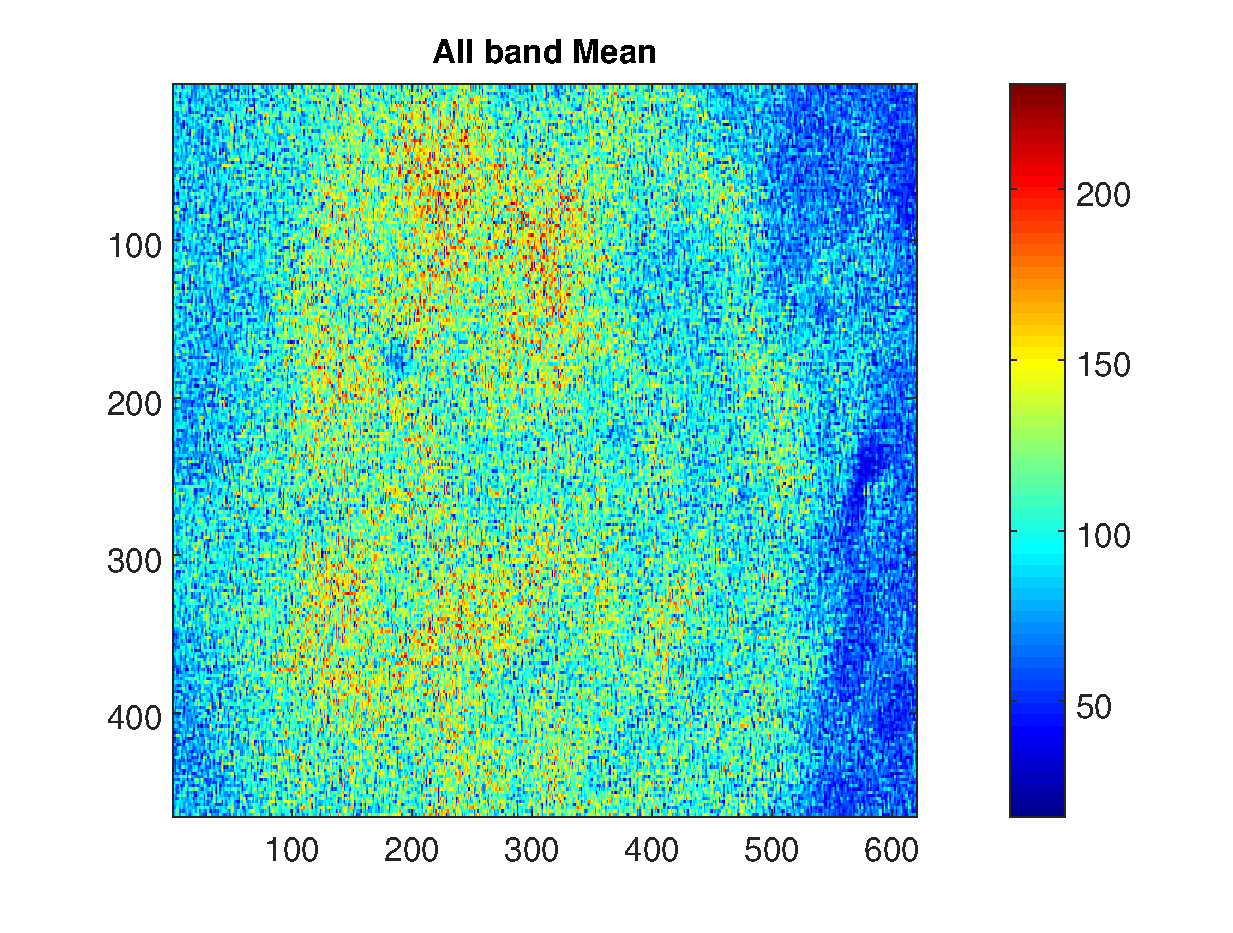
\includegraphics[width=0.85\columnwidth]{meanall.eps}
\caption{Light intensity distribution in the paper piece test.}
\label{fig:meanpaper}
\end{figure}

%%%%%%%%%%%%%%%%%%%%%%%%%%%%%%%%%%%%%%%%%%%%%%%%%%%%%%%%%%%%%%%%%%%%%%%%%%%%%%%%%%%%%%%%%
%%%%%%%%%%%%%%%%%%%%%%%%%%%%%%%%%%%%%%%%%%%%%%%%%%%%%%%%%%%%%%%%%%%%%%%%%%%%%%%%%%%%%%%%%
\section{Numerical analysis}
\label{sec:analysis}

\subsection{Data package filtering in three frequency band}
\label{subsec:firfilters}
Each data package or sub package ($P_T$) goes through of a filter bank with 4 outputs  having each
one a different type of processing, the first output is trivial because it
leave pass the information freely, this package is called of $P_T$, the others 3 processing types
return  signals, filter by frequency band; thus, 
we have the band between $[0,\frac{1}{3}]\frac{F_s}{2}$ (low frequencies),
the band between $[\frac{1}{3},\frac{2}{3}]\frac{F_s}{2}$ (intermediate frequencies) and
the band between $[\frac{2}{3},1]\frac{F_s}{2}$ (high frequencies); obtaining at end, the packages 
$P_X$, $P_Y$ and $P_Z$, respectively; as can be seen in the  Fig. \ref{fig:firfilters}.
Internally the obtaining of the filtered packages are realized using in cascade
two low pass Finite Impulse Response ($FIR$) filters of order $32$, so that
the sum of signals $P_X+P_Y+P_Z=P_T$.
\begin{figure}[h!]
\centering
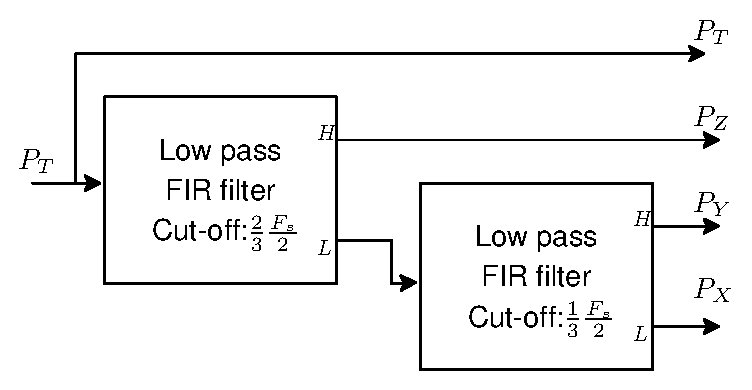
\includegraphics[width=0.55\columnwidth]{firfilters.eps}
\caption{Filtering of data packages.}
\label{fig:firfilters}
\end{figure}



\subsection{Temporal speckle deviation matrix}
\label{subsec:deviation}
The calculus of the temporal speckle deviation matrix ($\sigma$) \cite{Nothdurft:05} 
uses as input, the $N$ images of a data package.
We designate to each image, in the package $P$, as $\mathbf{I}_{k}$, $1\leq k \leq N$, being $k$ an integer;
thus, to get the value $\sigma$, 
 it is necessary to get 
the matrix $\sigma$ as seen in the Equation \ref{eq:cont2}, 
\begin{equation}\label{eq:cont2}
\sigma  = \sqrt{ \frac{1}{N} \sum_{k=1}^{N} (\mathbf{I}_{k}-\mu)^2  },
\end{equation}
being that, the value $\mu$ can be calculated as, 
\begin{equation}\label{eq:cont1}
\mu =  \frac{1}{N} \sum_{k=1}^{N} \mathbf{I}_{k},
\end{equation}


Additionally, can be defined the temporal speckle deviation index, $\bar{\sigma}=<\sigma>$, as the mean value
of all elements in $\sigma$, being $<.>$ the mean spatial operator.
%And $\sigma_p$ as any value of an element in  $\sigma$.

\subsection{Datapack processing in the ink drying test }
\label{subsec:numprocink}

As explicated in the Sec. \ref{sec:descriptionink} we have in the ink drying test, analysis regions  with
two levels of illumination in each data packages; thus, we  separate each package in two sub package
(left and right), representing each one the regions shown in the Fig. \ref{fig:regions}.
These sub packages are filtered following the process explicated in the Sec. \ref{subsec:firfilters},
obtaining the packages $P_T$, $P_X$, $P_Y$ and $P_Z$.
\begin{figure}[h!]
\centering
\includegraphics[width=0.65\columnwidth]{filtering.eps}
\caption{Filtering of data packages.}
\label{fig:filtering}
\end{figure}
Immediately later of obtained these filtered packages, over each one of these
is calculated the temporal speckle deviation matrix and in base of this result are obtained the 
temporal speckle deviation indexes $\bar{\sigma}_T$, $\bar{\sigma}_X$, $\bar{\sigma}_Y$ and
$\bar{\sigma}_Z$. The procedure to obtain these values is 
explicated in the Sec. \ref{subsec:deviation}.

\subsection{Statistical analysis of relation between the matrices $\sigma$ and $\mu$}
\label{subsec:statistical}
We define $\sigma_i$ and $\mu_i$
as the values in the $i-th$ position in the $\sigma$  
and $\mu$ matrices, respectively; also define $\mu_p$
as any element value in  $\mu$.
And finally we define the set $S_{\mu_p}=\{\sigma_i: \mu_i\equiv \mu_p; \forall i\}$
as the set of all $\sigma_i$  values given that $\mu_i\equiv\mu_p$.
With all these in mint we calculate the vectors $L_p$, $\sigma_p$ and
$e_p$ using all the $\mu_p$ values, according the next description.
\begin{itemize}
 \item $L_p(\mu_p)=card\left(S_{\mu_p}\right)$,  being $L_p(\mu_p)$ the number of elements
 in the set $S_{\mu_p}$ and $card(.)$ the cardinality function operator.
 \item $\sigma_p(\mu_p)=mean\left(S_{\mu_p}\right)$, being $\sigma_p(\mu_p)$
 the mean value of elements in the set $S_{\mu_p}$ and $mean(.)$ represents the mean value function operator.
 \item $e_p(\mu_p)=std\left(S_{\mu_p}\right)$, being $\e_p(\mu_p)$
 the standard  deviation value of elements in the set $S_{\mu_p}$ and $std(.)$ represents the standard deviation function operator.
\end{itemize}
In the practice only will be take in count in the vectors, values of $\mu_p$
with a $L_p(\mu_p)>200$ samples, to establish a limit to consider a set of representative samples.


\subsection{Datapack processing in the paper piece test }
\label{subsec:numprocink}

As explicated in the Sec. \ref{sec:descriptionpaper}, in this test we have one data package;
this package is filtered following the process explicated in the Sec. \ref{subsec:firfilters},
obtaining the packages $P_T$, $P_X$, $P_Y$ and $P_Z$,
over each one of these filtered packages 
are calculated the temporal speckle mean matrix and the 
temporal speckle deviation matrix, as can be seen in the Fig. \ref{fig:filtering2}.

\begin{figure}[h!]
\centering
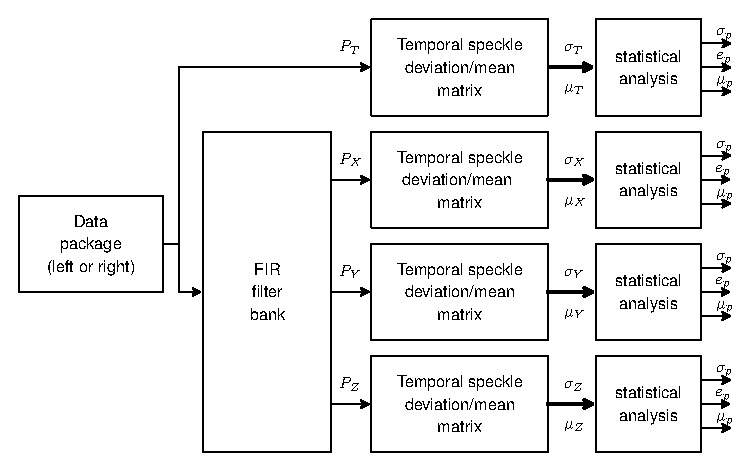
\includegraphics[width=0.65\columnwidth]{filtering2.eps}
\caption{Filtering of data package in paper piece test.}
\label{fig:filtering2}
\end{figure}

In base of these results are made statistical analysis to obtain the 
vectors $\sigma_p$, $\mu_p$, $e_p$ to each one of bands. 
The procedure to obtain these values is explicated in the Sec. \ref{subsec:statistical}.


%%%%%%%%%%%%%%%%%%%%%%%%%%%%%%%%%%%%%%%%%%%%%%%%%%%%%%%%%%%%%%%%%%%%%%%%%%%%%%%%%%%%%%%%%
%%%%%%%%%%%%%%%%%%%%%%%%%%%%%%%%%%%%%%%%%%%%%%%%%%%%%%%%%%%%%%%%%%%%%%%%%%%%%%%%%%%%%%%%%
\section{Numerical results} 
\label{sec:numerical}

\subsection{Numerical results in the ink drying test} 
\label{subsec:numericalink}
In the Fig. \ref{fig:numerical} we can see the result of data packages processing 
 in the ink drying test. The Fig. \ref{fig:allink}
represent the $\bar{\sigma}_T$ value in two light intensity levels, It is calculates over the package $P_T$
trough the time, and use the complete frequency band.
The Fig. \ref{fig:stdxink}
represent the $\bar{\sigma}_X$ value in two light intensity levels, It is calculates over the package $P_X$
trough the time, and use the frequency band between $0$ and $\frac{1}{3}\frac{F_s}{2}$Hz.
The Fig. \ref{fig:stdyink}
represent the $\bar{\sigma}_Y$ value in two light intensity levels, It is calculates over the package $P_Y$
trough the time, and use the frequency band between $\frac{1}{3}\frac{F_s}{2}$ and $\frac{2}{3}\frac{F_s}{2}$ Hz.
And the Fig. \ref{fig:stdzink}
represent the $\bar{\sigma}_Z$ value in two light intensity levels, It is calculates over the package $P_Z$
trough the time, and use the frequency band between $\frac{2}{3}\frac{F_s}{2}$ and $\frac{F_s}{2}$ Hz.
\begin{figure}[h!]
    \centering
    \begin{subfigure}[b]{0.475\textwidth}
        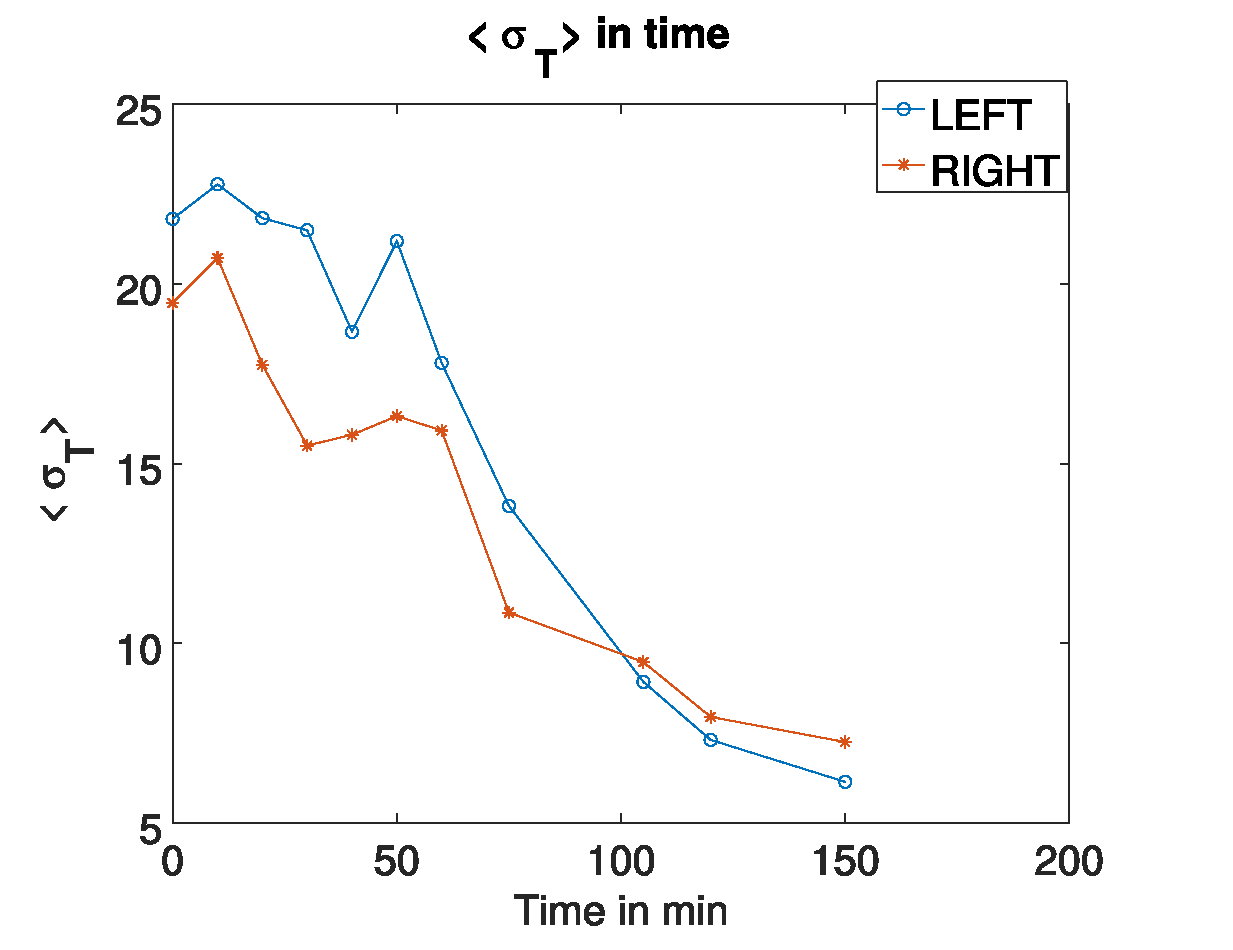
\includegraphics[width=\textwidth]{std-all.eps}
	\caption{$\bar{\sigma}_T$ value through  the time.}
        \label{fig:allink}
    \end{subfigure}
    ~
    \begin{subfigure}[b]{0.475\textwidth}
        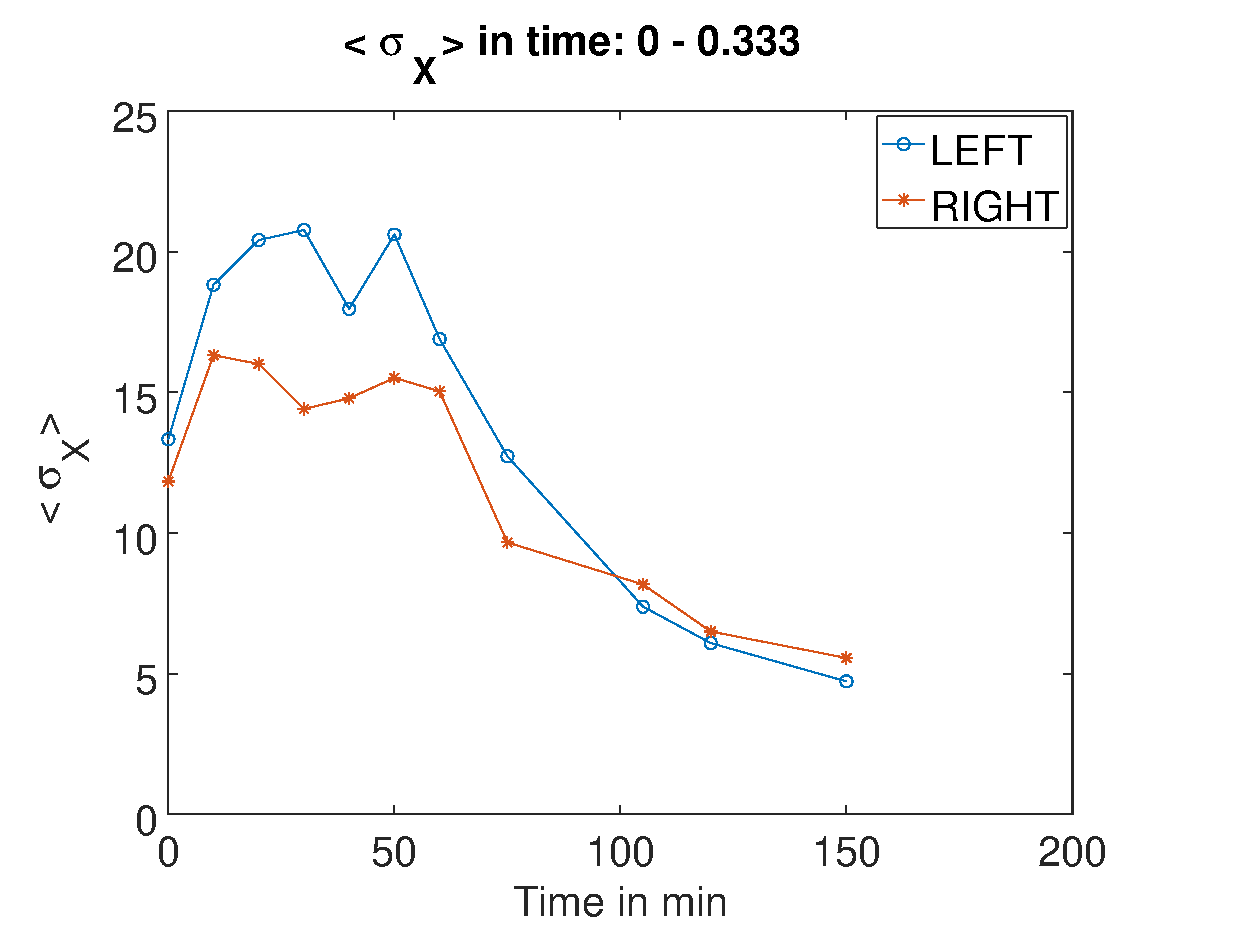
\includegraphics[width=\textwidth]{std-bandx.eps}
	\caption{$\bar{\sigma}_X$ value through  the time.}
        \label{fig:stdxink}
    \end{subfigure}
    ~\\ 
    \begin{subfigure}[b]{0.475\textwidth}
        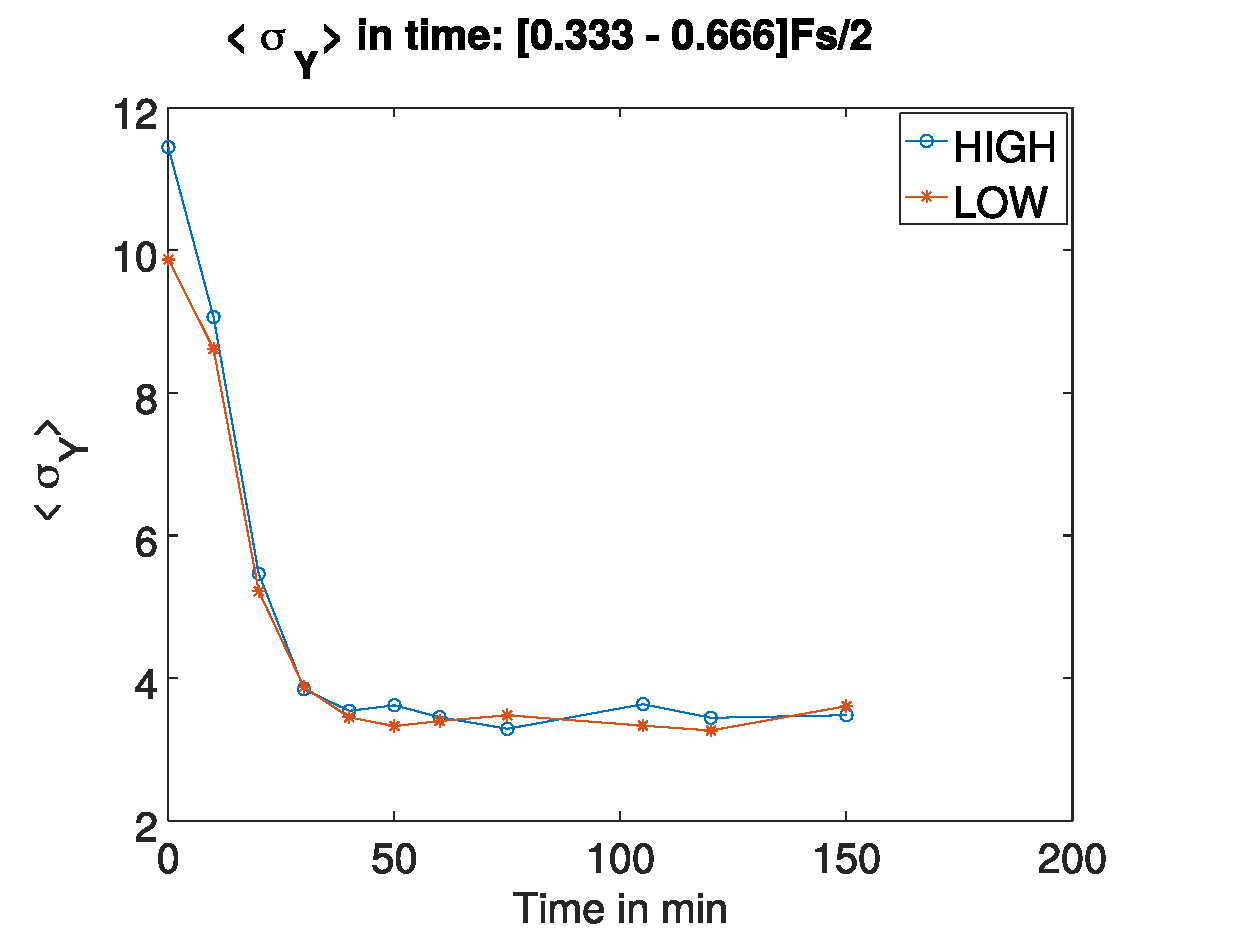
\includegraphics[width=\textwidth]{std-bandy.eps}
	\caption{$\bar{\sigma}_Y$ value through  the time.}
        \label{fig:stdyink}
    \end{subfigure}
  ~
    \begin{subfigure}[b]{0.475\textwidth}
        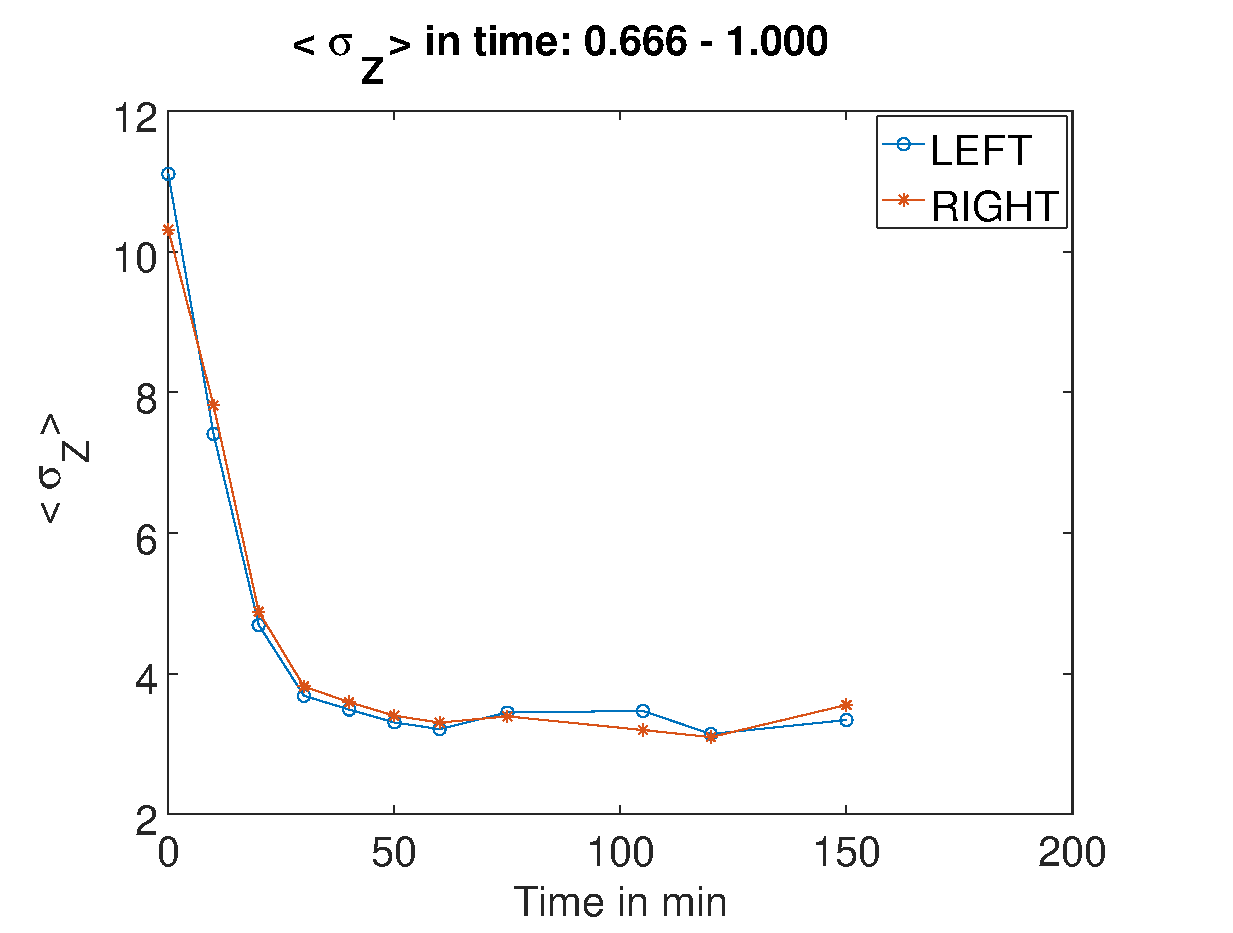
\includegraphics[width=\textwidth]{std-bandz.eps}
	\caption{$\bar{\sigma}_Z$ value through  the time.}
        \label{fig:stdzink}
    \end{subfigure}
    
\caption{Numerical results in the ink drying test.}\label{fig:numerical}
\end{figure}
As can be seen, when analyze the index over the complete frequency band (Fig. \ref{fig:allink}),
we have different results to both illuminations levels, being that the index
value It is major in the left side,that is the side with most illumination. This 
indicates a positive influence of illumination level in the index value.
By other side, if we observe the figures \ref{fig:stdxink}, \ref{fig:stdyink} and \ref{fig:stdzink},
we can perceive as the index values from different
illuminations  turn most similar with the grow of frequency.
being greater this similarity in the frequency band between $\frac{2}{3}\frac{F_s}{2}$ and $\frac{F_s}{2}$ Hz.
Thus the similarity is limit by the sampling frequency used.

Finally It is important highlight that in an ink drying test, like the used here,
It is characterized by speckle signals with high frequencies in the begin time
of drying and  speckle signals with low frequencies at end, being gradual this frequency transition
until reach the limit of signal and to have only the noise of test.
So that, when in the figures It is observe a horizontal line in the index, these data
should not be use in the comparisons, even if they are similar, given that these
only are show the noise of test. By example, in the Fig. \ref{fig:stdzink}
we filter so that only have high frequency signals; later, we know that these only happen
in the begin of drying process, and in the figure this happen from 0 until
the 50 minutes and later only have a similar horizontal line in both illuminations.
This indicates that the comparisons of index illumination independence
only should be made between these minutes because out this range we will be using
the noise of test in the comparisons.

\subsection{Numerical results in the paper piece test} 
\label{subsec:numericalpaper}
In the Fig. \ref{fig:papelstd} we can see the result of the processing 
the data packages in the paper piece test. The Fig. \ref{fig:papelall}
represent the $\sigma_T$ matrix that use the complete frequency band.
The Fig. \ref{fig:papelstd_stdx}
represent the $\sigma_X$ matrix that use the frequency band between $0$ and $\frac{1}{3}\frac{F_s}{2}$Hz.
The Fig. \ref{fig:papelstd_stdy}
represent the $\sigma_Y$ matrix that use the frequency band between $\frac{1}{3}\frac{F_s}{2}$ and $\frac{2}{3}\frac{F_s}{2}$ Hz.
And the Fig. \ref{fig:papelstd_stdz} 
represent the $\sigma_Z$ matrix that use the frequency band between $\frac{2}{3}\frac{F_s}{2}$ and $\frac{F_s}{2}$ Hz.
\begin{figure}[h!]
    \centering
    \begin{subfigure}[b]{0.485\textwidth}
        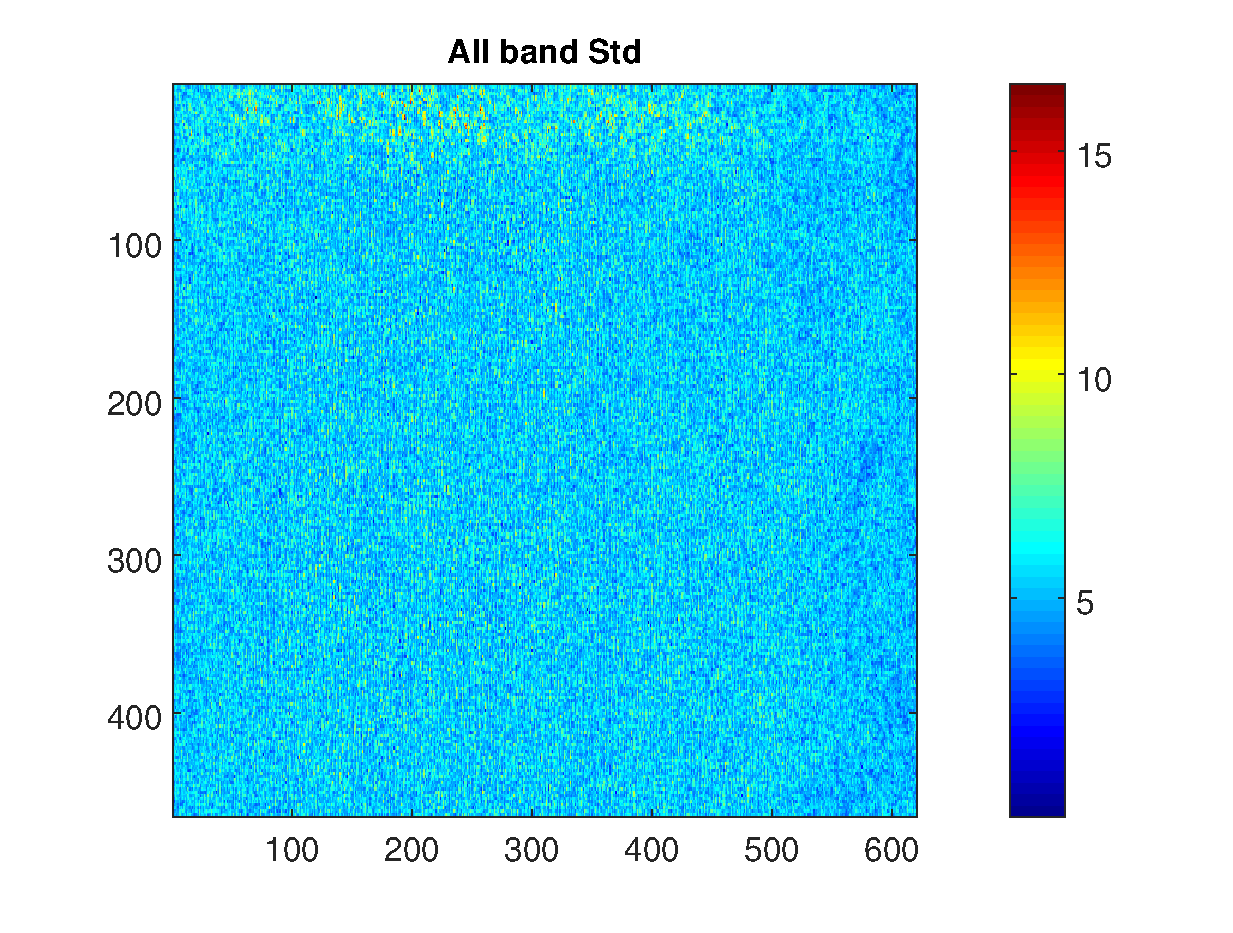
\includegraphics[width=\textwidth]{stdall.eps}
	\caption{$\sigma_T$ matrix over the complete frequency band.}
        \label{fig:papelall}
    \end{subfigure}
    ~
    \begin{subfigure}[b]{0.465\textwidth}
        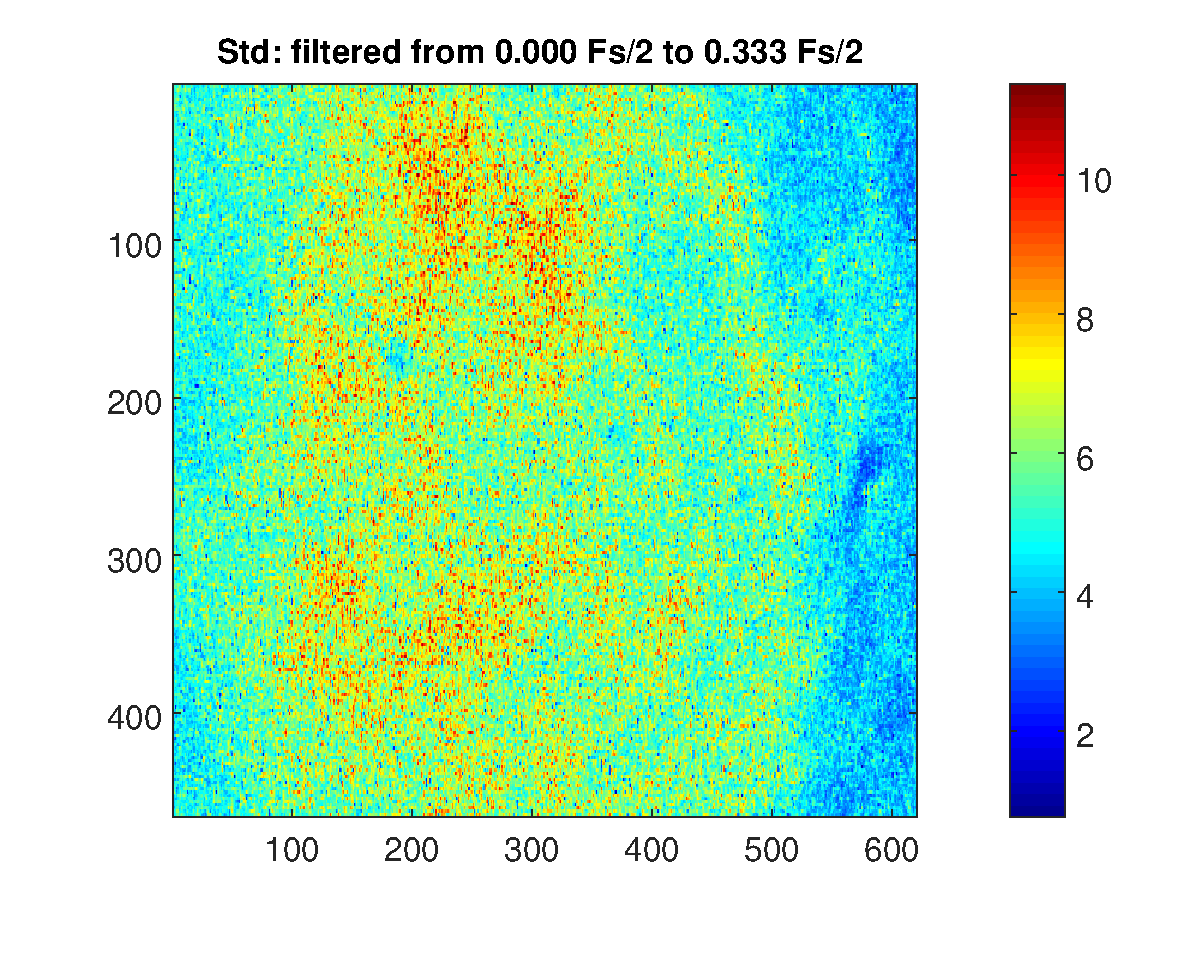
\includegraphics[width=\textwidth]{stdx.eps}
	\caption{$\sigma_X$ matrix over the inferior third of the frequency band.}
        \label{fig:papelstd_stdx}
    \end{subfigure}
    ~\\ 
    \begin{subfigure}[b]{0.475\textwidth}
        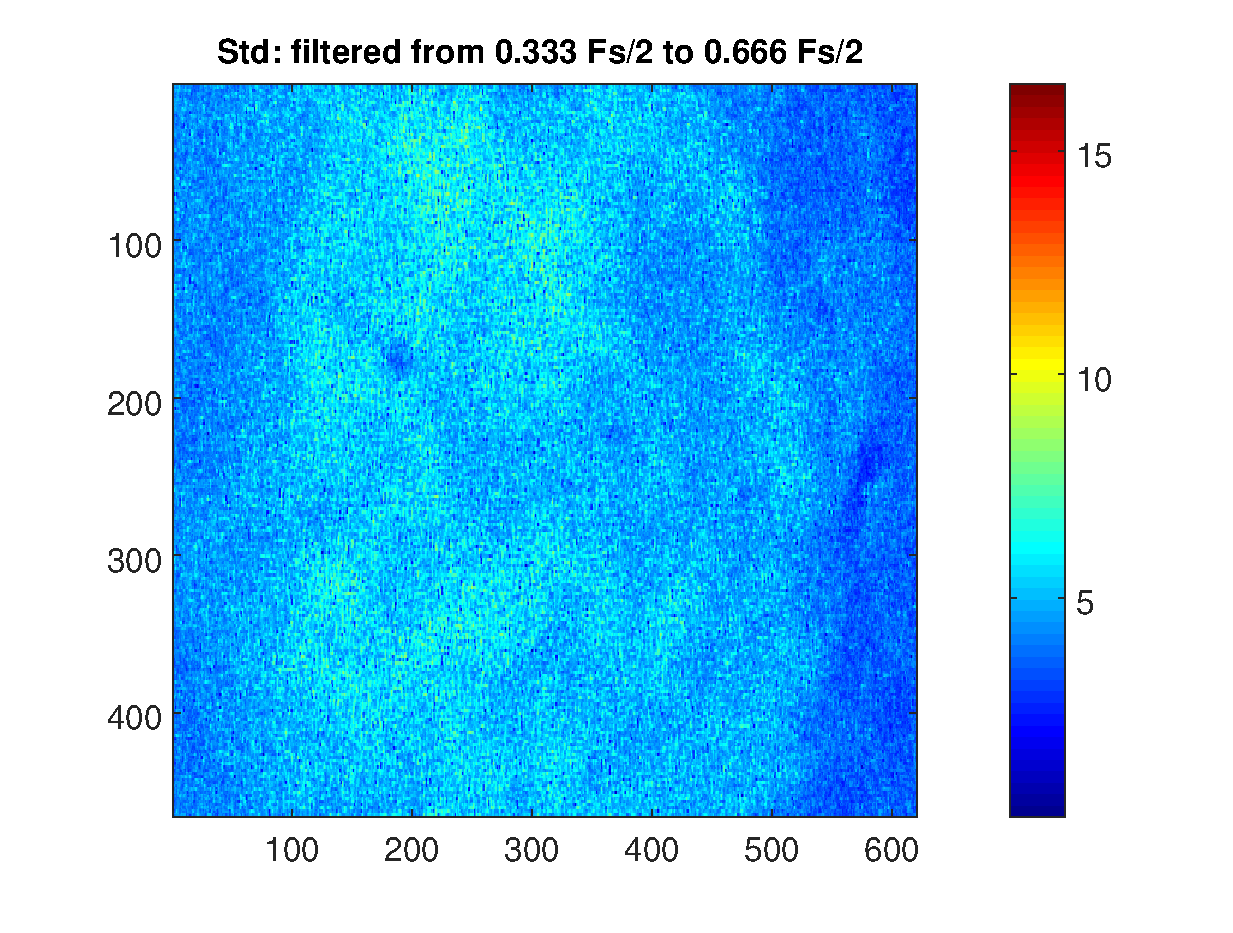
\includegraphics[width=\textwidth]{stdy.eps}
	\caption{$\sigma_Y$ matrix over the middle third of the frequency band.}
        \label{fig:papelstd_stdy}
    \end{subfigure}
  ~
    \begin{subfigure}[b]{0.475\textwidth}
        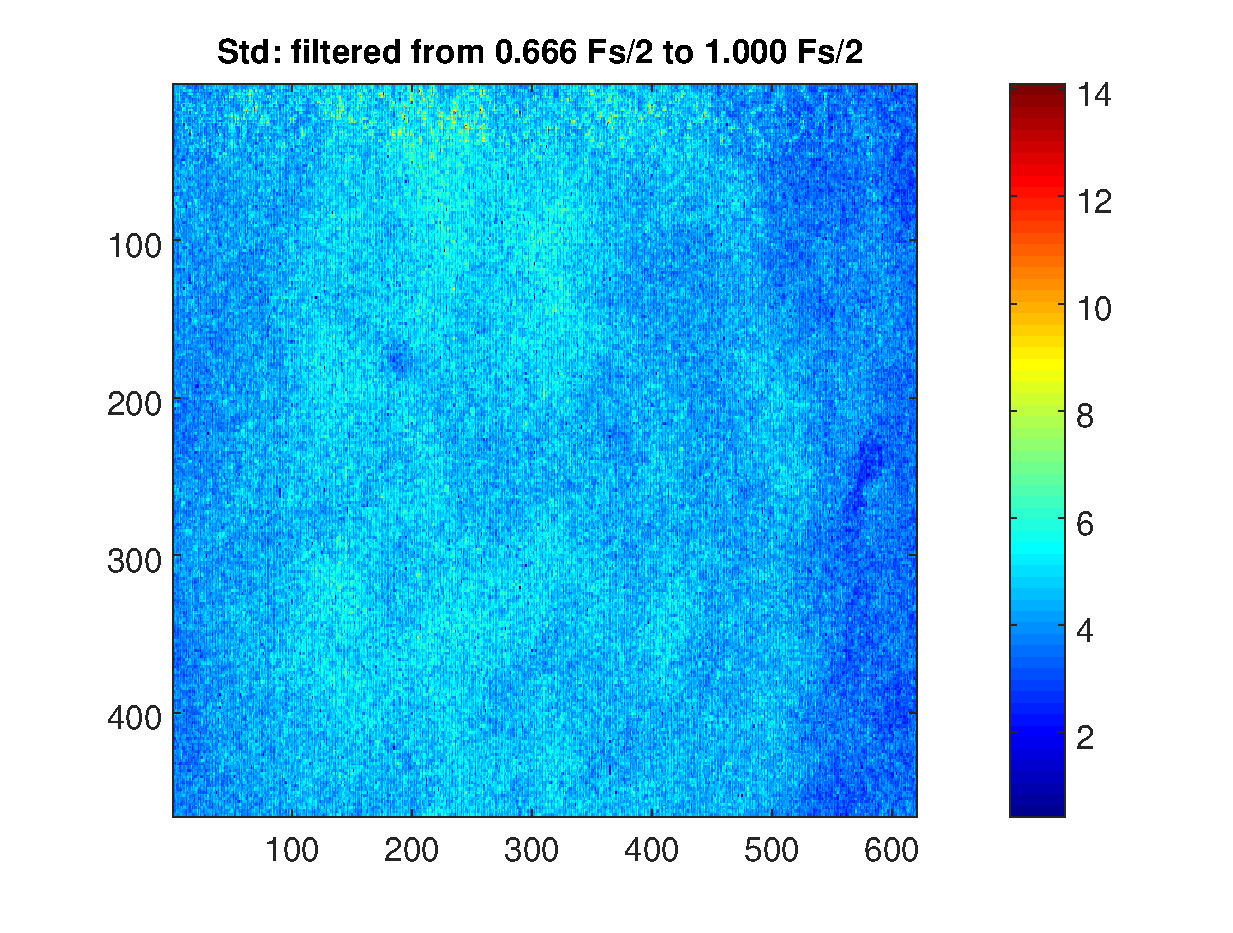
\includegraphics[width=\textwidth]{stdz.eps}
	\caption{$\sigma_Z$ matrix over the superior third of the frequency band.}
        \label{fig:papelstd_stdz}
    \end{subfigure}
    
    \caption{Temporal speckle deviation matrix of paper piece.}
    \label{fig:papelstd}
\end{figure}


In the next group of graphics we analysis the relation between a value $\sigma_p$,
in the $\sigma$ matrix, with a value $\mu_p$, in the $\mu$ matrix, to all
frequency bands. 
These analysis have importance because  the value $\mu_p$
is related with the illumination level in the surface of sample \cite{Nothdurft:05}
and the color or material of sample. Thus, when we choose $\mu_p$  as reference variable
in a homogeneous sample,  
in true we choose indirectly the illumination level in the surface.
In these sense, the Figs. \ref{fig:papelilllevel}, \ref{fig:illlevel_stdx}, \ref{fig:illlevel_stdy}
and \ref{fig:illlevel_stdz} show the variables $\sigma_p$, $e_p$ and $L_p$ in function
of  $\mu_p$, to the case of the complete frequency band, the inferior third of the frequency band,
the middle third of the frequency band and the superior third of the frequency band,
respectively in each sub figure. It is import to note that $e_p$ ever is graph as percentage
in the relation to the value $\sigma_p$, this means  $100 \frac{e_p}{\sigma_p} \%$.
\begin{figure}[h!]
    \centering
    \begin{subfigure}[b]{0.475\textwidth}
        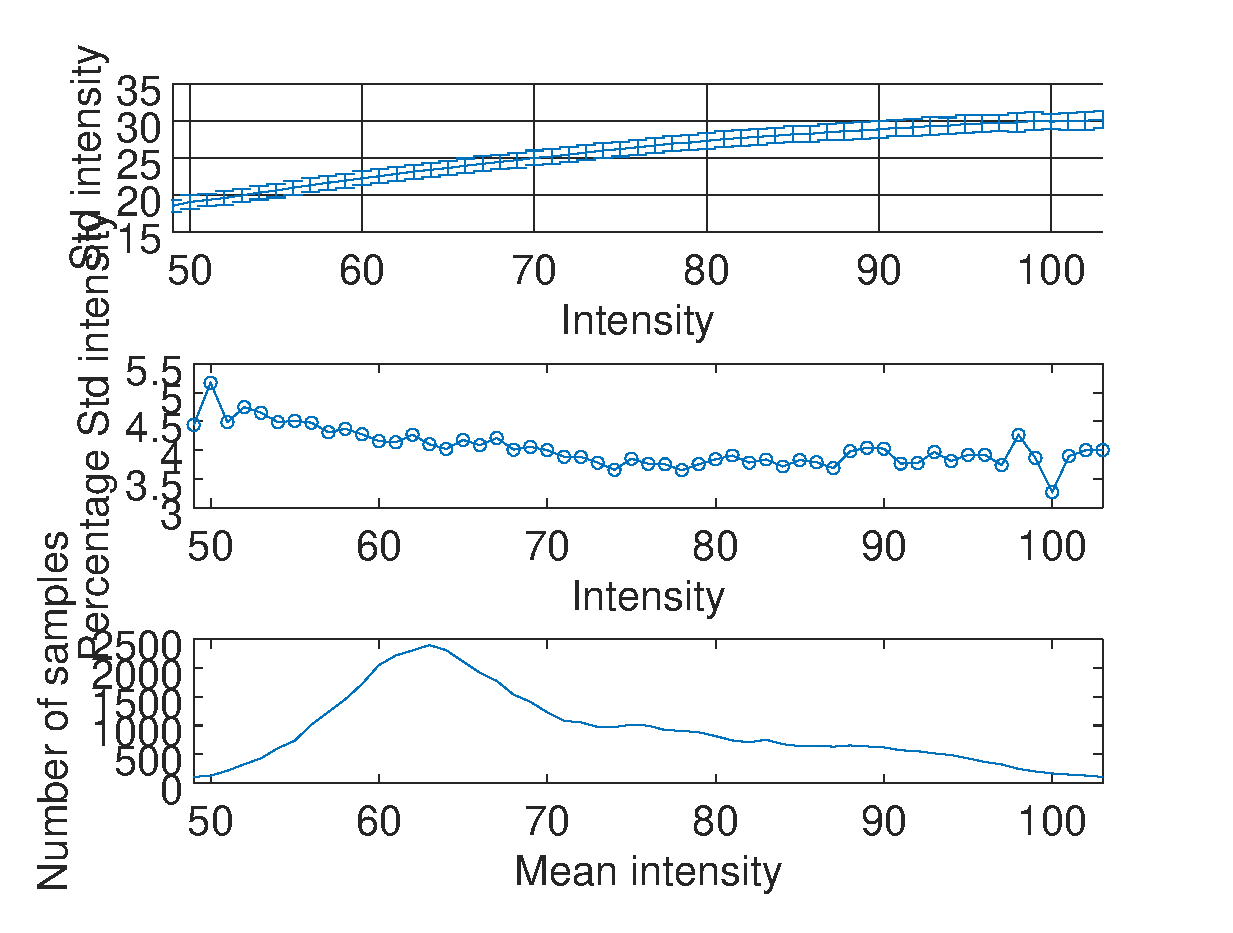
\includegraphics[width=\textwidth]{stdall_curve.eps}
	\caption{Analysis in the complete frequency band.}
        \label{fig:illlevel_all}
    \end{subfigure}
    ~
    \begin{subfigure}[b]{0.475\textwidth}
        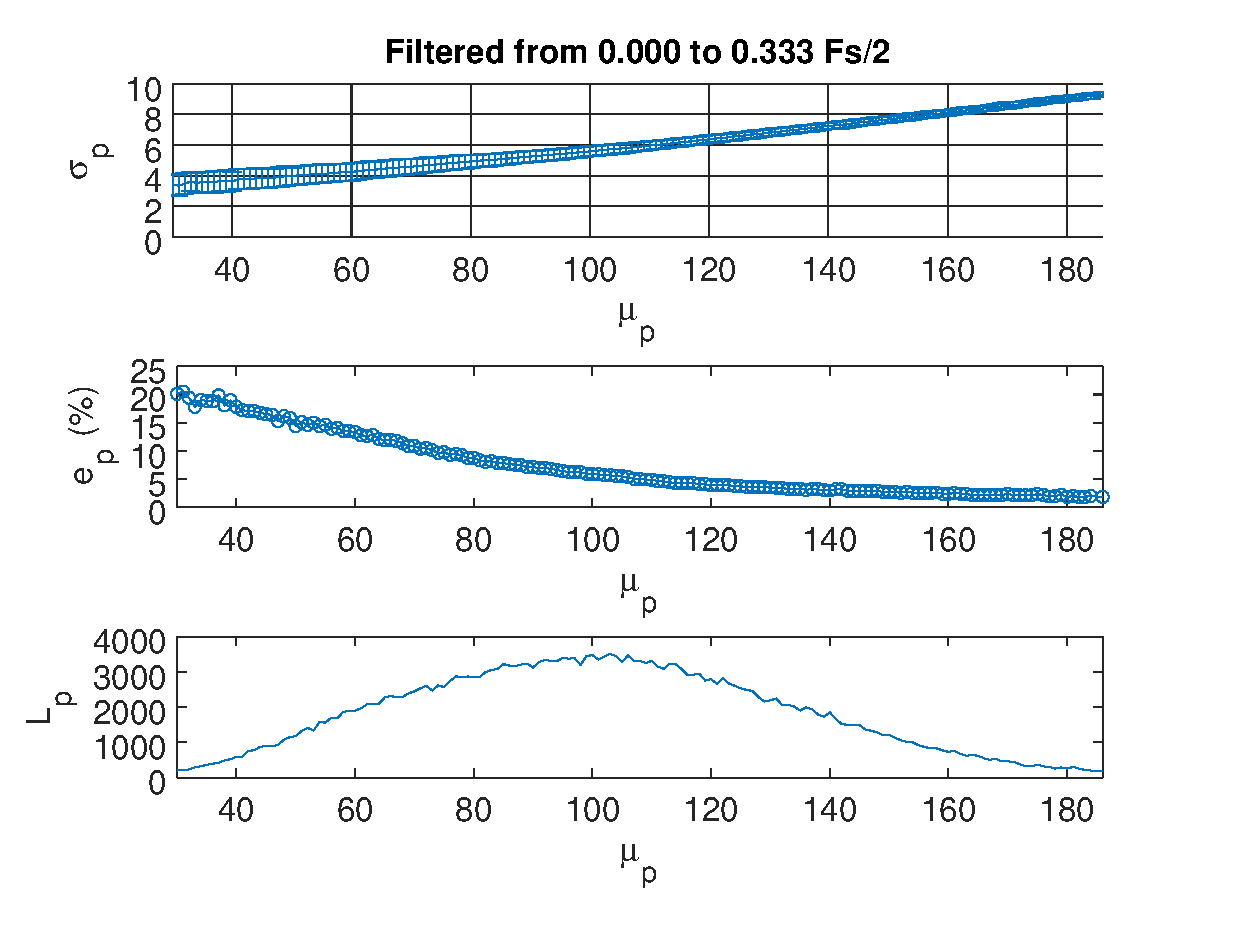
\includegraphics[width=\textwidth]{stdx_curve.eps}
	\caption{Analysis in the inferior third of the frequency band.}
        \label{fig:illlevel_stdx}
    \end{subfigure}
    ~\\ 
    \begin{subfigure}[b]{0.475\textwidth}
        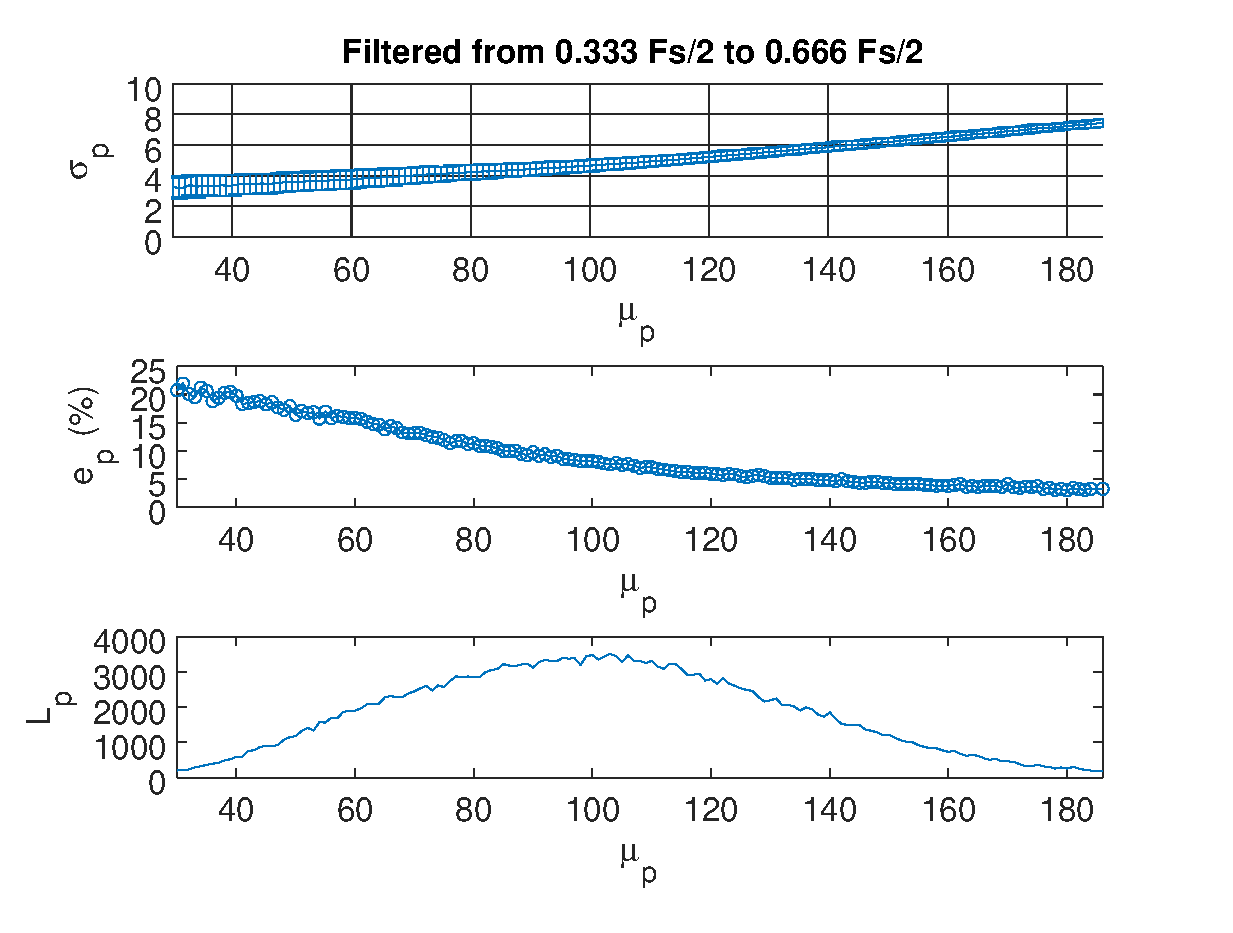
\includegraphics[width=\textwidth]{stdy_curve.eps}
	\caption{Analysis in the middle third of the frequency band.}
        \label{fig:illlevel_stdy}
    \end{subfigure}
  ~
    \begin{subfigure}[b]{0.475\textwidth}
        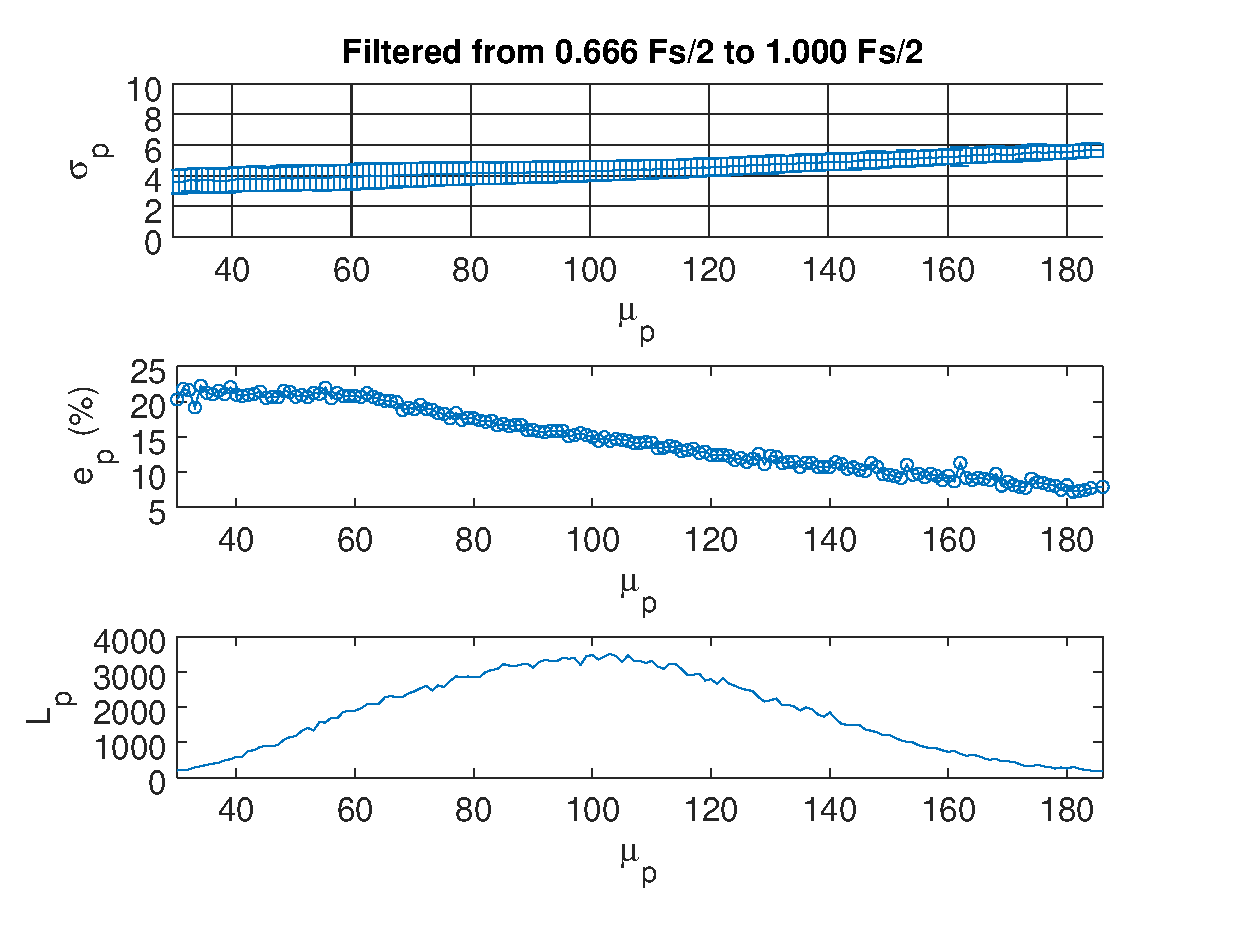
\includegraphics[width=\textwidth]{stdz_curve.eps}
	\caption{Analysis in the superior third of the frequency band.}
        \label{fig:illlevel_stdz}
    \end{subfigure}
    
    \caption{Relation between the standard deviation value and the illumination level in a paper piece.}
    \label{fig:papelilllevel}
\end{figure}

In all these results we hope see a homogeneous tend in the index values,
in all spatial positions, because has been analyzed an homogeneous paper piece.
Keeping this in mind, in the Fig. \ref{fig:papelall} we observe
a  slightly homogeneity in the values because exist a variability in 
the result in some regions, this is most evident if we analyze the Fig. \ref{fig:illlevel_all}
where observe as change the value $\sigma_p$ in relation to the value $\mu_p$,
so that
$\sigma_p$ is around of $5.5$ with changes that depended of illumination level $\mu_p$,
but even to a specific value $\mu_p$ exist much variability in the expected value of $\sigma_p$,
having a $e_p$ around of $12\%$ in the best case. In other cases in the Figs. \ref{fig:illlevel_stdx},
\ref{fig:illlevel_stdy} and \ref{fig:illlevel_stdz}. We observe a linear ascendant relation
between $\sigma_p$ and $\mu_p$, being that the slope decreases with 
the increase of the frequency band. As can be seen in the Fig. \ref{fig:illlevel_stdz}
where the variations in $\mu_p$  only slightly influence to $\sigma_p$ and the error $e_p$
can be of $5\%$ when the illumination is maximum. 

%%%%%%%%%%%%%%%%%%%%%%%%%%%%%%%%%%%%%%%%%%%%%%%%%%%%%%%%%%%%%%%%%%%%%%%%%%%%%%%%%%%%%%%%%
%%%%%%%%%%%%%%%%%%%%%%%%%%%%%%%%%%%%%%%%%%%%%%%%%%%%%%%%%%%%%%%%%%%%%%%%%%%%%%%%%%%%%%%%%
\section{Conclusion} 

In this work were presented comparisons between the values of the temporal speckle 
deviation index to 3 different frequency bands of the speckle signal and
different illuminations levels, in a
dynamic laser speckle analysis, the results shown as the influence of illumination level over
the index decreases with the use of signals with high frequency bands.


\section{Acknowledgment}
We wish to acknowledge the partial financial support for this study provided by the $CAPES$ 
scholarship
$PNPD$ Program, $FAPEMIG$ and $CNPQ$.

%----------------------------------------------------------------------------------------
%	REFERENCE LIST
%----------------------------------------------------------------------------------------
\section{Bibliography}
\bibliography{report}   %>>>> bibliography data in report.bib
\bibliographystyle{spiebib}   %>>>> makes bibtex use spiebib.bst


%----------------------------------------------------------------------------------------

\end{document} 


